\documentclass[a4paper]{article}

\usepackage[utf8]{inputenc}
\usepackage{indentfirst}
\usepackage{float}
\usepackage{geometry}
\usepackage{polski}
\usepackage{mathtools}
\usepackage{tcolorbox}
\usepackage{listings}
\usepackage{amssymb}
\usepackage[none]{hyphenat}
\usepackage{tabularx}

\lstset{frame=tb,
  language=Java,
  aboveskip=3mm,
  belowskip=3mm,
  showstringspaces=false,
  columns=flexible,
  basicstyle={\small\ttfamily},
  numbers=none,
  numberstyle=\tiny\color{rgb}{0.5,0.5,0.5},
  keywordstyle=\color{rgb}{0.58,0,0.82}
  commentstyle=\color{rgb}{0,0.6,0},
  stringstyle=\color{mauve},
  breaklines=true,
  breakatwhitespace=true,
  tabsize=3
}
\renewcommand{\familydefault}{\sfdefault}
\newcommand\tab[1][1cm]{\hspace*{#1}}

\title{\textbf{VaccDistributor}}
\author{Kamil Sztandur}
\date{07/11/2020}
\begin{document}
\begin{tcolorbox}
\maketitle
\end{tcolorbox}
\newpage

\section*{Rozdział 1: OPIS OGÓLNY}
\subsection*{Podrozdział 1.1: Nazwa programu.}
\tab Program nazywa się \textbf{VaccDistributor}.
\subsection*{Podrozdział 1.2: Poruszany problem.}
\tab Problemem rozwiązywanym przez ten program jest zagadnienie jak najbardziej optymalnego pod kątem ekonomicznym rozdysponowania szczepionek pomiędzy poszczególnymi dostawcami, a aptekami, na podstawie podanych przez użytkownika połączeń. Program skupia się na tym, aby koszt dystrybucji szczepionek był jak najmniejszy. Nie gwarantuje, że zapotrzebowanie każdej apteki zostanie zaspokojone. Także jest to wariant egoistyczny.
\subsection*{Podrozdział 1.3: Użytkownik docelowy.}
\tab Użytkownikiem naszego programu powininna być grupa menadżerska odpowiedzialna za dystrybucję szczepionek. Program stanowi proste rozwiązanie jak najbardziej optymalnego ekonomicznie rozwiązania problemu. 
\newline

\section*{Rozdział 2: OPIS FUNKCJONALNOŚCI}
\subsection*{Podrozdział 2.1: Jak korzystać z programu?}
\tab Uruchomienie programu ze względu na brak oprawy graficznej może sprawiać trudności mniej wtajemniczonym w komputery użytkownikom. Program uruchamia się z poziomu terminalu systemu operacyjnego, na którym jest zainstalowana najnowsza wersja oprogramowania Java. 

\subsection*{Podrozdział 2.2: Uruchomienie programu.}
\tab Aby uruchomić program wystarczy wpisać komendę w terminalu systemu operacyjnego spełniającego opisane wymagania:
\begin{lstlisting}
	java -jar vaccDistributor.jar input.txt
\end{lstlisting}
znajdując się w katalogu, w którym umieszczone zostały równocześnie plik programu \textbf{vaccDistributor.jar} oraz tekstowy plik wejściowy z danymi (tutaj \textbf{input.txt}). Należy pamiętać o dopisaniu rozszerzenia pliku. Sama nazwa (tutaj \textbf{input}) nie pozwoliłaby na odnalezienie wskazanego pliku. \newline \newline
\tab Należy dokładnie przestudiować strukturę pliku wejściowego na podstawie poniższego przykładu, ponieważ wszelkie odstępstwa od ogólnoprzyjętego szablonu mogą spowodować nieprawidłową pracę, a nawet zatrzymanie pracy programu. Tekstowy plik wejściowy powinien zawierać trzy nagłówki, oznaczające kolejno listy producentów, aptek i dostępnych połączeń. Kolejne parametry w linijce powinny być oddzielna ciągiem znaków " $|$ ". Nie należy powielać nagłówków ani umieszczać ich w innej kolejności.
 
\newpage
\subsection*{Podrozdział 2.3: Przykładowy plik wejściowy.}
\begin{tcolorbox}
\# Producenci szczepionek (id | nazwa | dzienna produkcja)
\newline 0 $|$ BioTech 2.0 $|$ 900
\newline 1 $|$ EkoPolska 2020 $|$ 1300
\newline 2 $|$ Post-Covid Sp. z o.o. $|$ 1100
\newline \# Apteki (id $|$ nazwa $|$ dzienne zapotrzebowanie)
\newline 0 $|$ CentMedEko Centrala $|$ 450 
\newline 1 $|$ CentMedEko 24h $|$ 690 
\newline 2 $|$ CentMedEko Nowogrodzka $|$ 1200
\newline \# Połączenia producentów i aptek (id producenta $|$ id apteki $|$ dzienna maksymalna liczba dostarczanych szczepionek $|$ koszt szczepionki [zł] )
\newline 0 $|$ 0 $|$ 800 $|$ 70.5 
\newline 0 $|$ 1 $|$ 600 $|$ 70 
\newline 0 $|$ 2 $|$ 750 $|$ 90.99
\newline 1 $|$ 0 $|$ 900 $|$ 100 
\newline 1 $|$ 1 $|$ 600 $|$ 80
\newline 1 $|$ 2 $|$ 450 $|$ 70
\newline 2 $|$ 0 $|$ 900 $|$ 80
\newline 2 $|$ 1 $|$ 900 $|$ 90
\newline 2 $|$ 2 $|$ 300 $|$ 100
\end{tcolorbox}

\newpage
\section*{Rozdział 3: FORMATY DANYCH I STRUKTURA PLIKÓW.}
\subsection*{Podrozdział 3.1: Pojęcia i obiekty dziedziny aplikacji (słownik dziedziny).}

\begin{enumerate}
    \item \textbf{Producent (in. dostawca, "supplier"):}
          \begin{itemize}
              \item \textbf{ID -} numer identyfikacyjny producenta na liście. Musi być unikatowy.
              \item \textbf{Nazwa ("name")-} nazwa producenta. Musi być unikatowa.
			\item \textbf{Dzienna produkcja ("daily production") -} Ilość dostępnych codziennie szczepionek gotowych do dystrybucji do aptek.
			\item \textbf{Dostępna dzienna produkcja ("available daily production") -} aktualna ilość dostępnych szczepionek gotowych do dystrybucji do aptek. Od poprzedniego parametru różni się tym, że uwzględnia już podpisane umowy na dowóz określonej ilości do niektórych placówek.
          \end{itemize}
	
    \item \textbf{Apteka (in. placówka, "pharmacy"):}
          \begin{itemize}
              \item \textbf{ID -} numer identyfikacyjny apteki na liście. Musi być unikatowy.
              \item \textbf{Nazwa ("name")-} nazwa placówki apteki. Musi być unikatowa.
			\item \textbf{Dzienne zapotrzebowanie ("daily production") -} ilość szczepionek, która musi być dostarczana dziennie, aby zaspokoić potrzeby placówki.
			\item \textbf{Obecne dziennie zapotrzebowanie ("current daily need") -} aktualna ilość pozostałych szczepionek, która musi być dostarczana dziennie, aby zaspokoić potrzeby placówki. Uwzględnia umowy już podpisane na dostarczenie pewnej ilości i odejmuje je od domyślnego dziennego zapotrzebowania.
          \end{itemize}
	\item \textbf{Połączenie ("connection"):}
          \begin{itemize}
              \item \textbf{ID dostawcy ("supplier ID") -} numer identyfikacyjny dostawcy, od którego wychodzi dane połączenie.
			\item \textbf{ID apteki ("pharmacy ID") -} numer identyfikacyjny apteki, do której dochodzi dane połączenie.
              \item \textbf{Maksymalny transfer ("max transfer") -} maksymalna liczba szczepionek, która może zostać przewieziona jednego dnia tym połączeniem.
			\item \textbf{Pozostały transfer ("available transfer") -} pozostała liczba szczepionek, która może zostać przewieziona jednego dnia tym połączeniem. Uwzględnia już podpisane umowy na dowożenie tym połączeniem pewnej ilości szczpeionek.
			\item \textbf{Koszt pojedynczej szczepionki ("cost per single vaccine") -} koszt dostarczenia pojedynczej szczepionki tym połączeniem.
		\end{itemize}
	\item \textbf{Transakcja ("transaction").} Transakcja jest połączeniem o parametrach, które program uznał za najbardziej możliwie optymalne. W przeciwieństwie do listy wszystkich połączeń, transakcja jest połączeniem, które na pewno zostanie zrealizowane i jest opracowywane w trakcie pracy programu:
          \begin{itemize}
              \item \textbf{ID dostawcy ("supplier ID") -} numer identyfikacyjny dostawcy, od którego wychodzi dane połączenie.
			\item \textbf{ID apteki ("pharmacy ID") -} numer identyfikacyjny apteki, do której dochodzi dane połączenie.
              \item \textbf{Transfer ("max transfer") -} ilość szczepionek, która zostanie dostarczona tym połączeniem.
			\item \textbf{Koszt pojedynczej szczepionki ("cost per single vaccine") -} koszt dostarczenia pojedynczej szczepionki tym połączeniem.
			\item \textbf{Całkowity koszt ("total cost") -} całkowity koszt wykonania tej transakcji:
							\newline			
							\newline \tab $ \textbf{Całkowity koszt} = \textbf{Koszt pojedynczej szczepionki} \times \textbf{Transfer} $
          \end{itemize}
\end{enumerate}

\subsection*{Podrozdział 3.2: Struktura katalogów.}

\begin{figure}[H]
    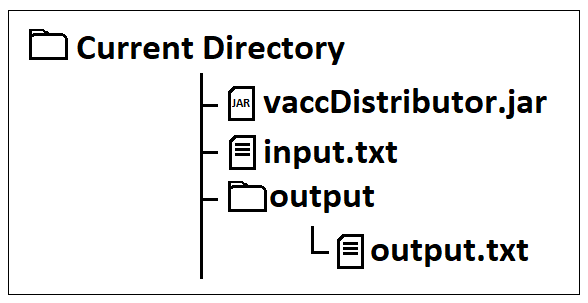
\includegraphics[width=10cm]{Katalogi.png}
    \centering
\end{figure}
\tab Plik wejściowy z danymi producentów, aptek i połączeń (tutaj \textbf{input.txt} powinien znajdywać się w tym samym katalogu co plik wykonywalny programu (tutaj \textbf{vaccDistributor.jar}). Po uruchomieniu programu zgodnie z instrukcjami opisanymi w poprzednim rozdziale zostanie utworzony podkatalog o nazwie \textbf{output}, w którym znajdzie się plik z optymalnym rozwiązaniem problemu \textbf{output.txt}.

\subsection*{Podrozdział 3.3: Przechowywanie danych w programie.}
\textbf{PRZYPOMNIENIE} Poprawne wywołanie programu:
\begin{lstlisting}
	java -jar vaccDistributor.jar input.txt
\end{lstlisting}


Zgodnie z poprawnym wywołaniem i przebiegem pracy programu powinien wyświetlić się taki komunikat. Symbolizować on będzie zakończenie pracy programu i pomyślne umieszczenie pliku z rozwiązaniem w podkatalogu output:
\begin{tcolorbox}
home:\$	java -jar vaccDistributor.jar input.txt
\newline Czytanie danych wejściowych... Sukces.
\newline Znajdywanie najlepszych połączeń... Sukces.
\newline Tworzenie katalogu z rozwiazaniem... Sukces.
\newline Zapisywanie danych wyjściowych do pliku... Sukces.
\newline 
\newline Praca programu zakończona pomyślnie.
\end{tcolorbox}

\newpage
W przypadku nie podania żadnego argumentu zostanie wyświetlony komunikat informujący o prawidłowym wywołaniu programu:
\begin{tcolorbox}
home:\$	java -jar vaccDistributor.jar
\newline Brak podanego pliku z danymi. Poprawne wywołanie:
\newline \tab java -jar vaccDistributor.jar input.txt
\newline gdzie input.txt to nazwa pliku z danymi, który znajduje się w biężącym katalogu.
\newline 
\newline Praca programu zakończona z błędem.
\end{tcolorbox}

W przypadku kiedy niewystarczająca wydajność producentów lub połączeń z aptekami nie jest w stanie zaspokoić ich wszystkich zostanie wyświetlony stosowny komunikat.
\begin{tcolorbox}
home:\$	java -jar vaccDistributor.jar input.txt
\newline Czytanie danych wejściowych... Sukces.
\newline [Ostrzeżenie] Producenci nie są dostatecznie wydajni dla tak wymagających aptek.
\newline Znajdywanie najlepszych połączeń... Sukces.
\newline Tworzenie katalogu z rozwiazaniem... Sukces.
\newline Zapisywanie danych wyjściowych do pliku... Sukces.
\newline 
\newline Praca programu zakończona pomyślnie.
\end{tcolorbox}

W przypadku podania nieistniejącego pliku zostanie wyświetlony stosowny komunikat:
\begin{tcolorbox}
home:\$	java -jar vaccDistributor.jar input.txt
\newline Czytanie danych wejściowych... Porażka. Podany plik nie istnieje.
\newline 
\newline Praca programu zakończona z błędem.
\end{tcolorbox}

W przypadku podania nieprawidłowego pliku zostaną wyświetlony komunikat zawierający przybliżony opis błędu:
\begin{tcolorbox}
home:\$	java -jar vaccDistributor.jar input.txt
\newline Czytanie danych wejściowych... Porażka. Podany plik jest nieprawidłowy.
\newline Opis błędu: Cost per single vaccine cannot be less than 0 at line 49.
\newline 
\newline Praca programu zakończona z błędem.
\end{tcolorbox}


\newpage
\subsection*{Podrozdział 3.4: Przykładowy plik wyjściowy.}
Plik wejściowy zawiera listę zleconych transakcji w formacie:
\begin{figure}[H]
    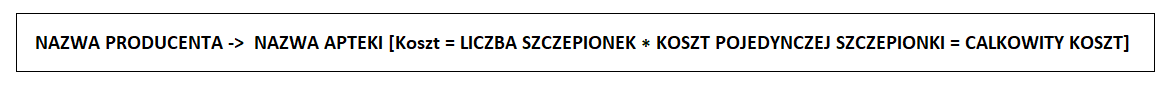
\includegraphics[width=14cm]{Output1.png}
    \centering
\end{figure}
Dodatkowo na końcu widnieje suma kosztów wszystkich transakcji poprzedzona stosowną etykietą \textbf{"Opłaty całkowite: "} po której zapisana zostaje suma kosztów wszystkich transakcji.\newline

\textbf{Przykładowy plik wyjściowy:}
\begin{tcolorbox}
BioTech 2.0 -$>$ CentMedEkoCentrala [Koszt = 300 * 70.5 = 21150 zł]
\newline EkoPolska 2020 -$>$ CentMedEkoCentrala [Koszt = 150 * 100 = 15000 zł]
\newline 
\newline /*...kolejne wiersze opisujące ustalone połączenia pomiędzy producentami, a aptekami...*/
\newline 
\newline Opłaty całkowite: 36150 zł
\end{tcolorbox}

\newpage
\section*{Rozdział 4: SCENARIUSZ DZIAŁANIA PROGRAMU.}
\subsection*{Podrozdział 4.2: Scenariusz ogólny.}
\begin{enumerate}
\item Przeczytanie wskazanego przez użytkownika pliku z danymi.
\item Obliczenie i utworzenie najbardziej optymalnych transakcji producenci - apteki.
\item Wypisywanie listy transakcji do pliku tesktowego w folderze \textbf{output}.
\end{enumerate}

\subsection*{Podrozdział 4.2: Scenariusz szczegółowy.}
\begin{enumerate}
\item Sprawdzenie, czy użytkownik podał jakiś plik wejściowy.
	\begin{itemize}
		\item Jeżeli nie, poinformuj go o tym, pokaż przykład prawidłowego wywołania i zakończ działanie.
	\end{itemize}
\item Sprawdzenie, czy plik podany przez użytkownika istnieje. 
	\begin{itemize}
		\item Jeżeli nie, poinformuj go o tym i zakończ działanie.
	\end{itemize}
\item Czytanie podanego pliku. Zczytywanie kolejnych producentów, aptek i połączeń do wewnętrznych kontenerów. Sprawdzanie składni na bieżąco. 
	\begin{itemize}
		\item Jeżeli składnia jest nieprawidłowa powiadom użytkownika, wskaż nr. linii i zakończ pracę.
		\item Jeżeli występują duplikaty, pomiń linię, wskaż jej numer i powiadom użytkownika potokiem błędu. Kontynuuj pracę programu.
	\end{itemize}
\item Oblicz, czy istnieją apteki, które nie mogą zostać w żaden sposób zaspokojone. 
	\begin{itemize}
		\item Jeżeli tak, to powiadom użytkownika o tej sytuacji. Kontynuuj pracę programu i zapamiętaj ten fakt dla algorytmu.
	\end{itemize}
\item Rozpocznij działanie algorytmu, tworzącego jak najtańsze połączenia dostawcy - apteki:
	\begin{itemize}
		\item Posortuj quicksortem listę połączeń rosnąco pod względem kosztu pojedynczej szczepionki.
		\item Duplikaty posortuj quicksortem malejąco pod względem rzeczywistego transferu. Za rzeczywisty transfer przyjmij najmniejszą liczbę z: 
		\begin{itemize}
				\item aktualne zapotrzebowanie apteki danego połączenia
				\item aktualnie dostępna liczba szczepionek u producenta danego połączenia
				\item aktualna przepustowość połączenia
		\end{itemize}
		\item Realizuj kolejne połączenia z początku listy w transakcje. W przypadku wyczerpania producenta, połączenia lub zaspokojenia apteki skreślaj z listy wszystkie pozycje je zawierające.
		\item Zwróć listę transakcji.
	\end{itemize}
\item Utwórz katalog output.
\item Utwórz plik output.txt w katalogu output i zapisz do niego zgodnie z szablonem listę utworzonych transakcji.
\item Poinformuj użytkownika o pomyślnym przebiegu programu. Zakończ działanie.
\end{enumerate}

\newpage
\subsection*{Podrozdział 4.3: Ekrany działania programu.}
Program przebiega w pełni w terminalu systemu operacyjnego, a na końcu wypisuje plik tekstowy w sposób zgodny z opisanym w poprzednich rozdziałach. Przykładowy ekran pracy programu wygląda w ten sposób:

Każde bieżąco wykonywane zadanie sygnalizowane jest opisem kończącym się trzema kropkami "..." i tekst pozostanie w takim stanie na ekranie dopóki nie zostanie ono zakończone lub przerwane z powodu błędu. Wówczas zaraz po trzech kropkach zostanie wypisany stan zadania.

\begin{tcolorbox}
home:\$	java -jar vaccDistributor.jar input.txt
\newline Czytanie danych wejściowych... 
\end{tcolorbox}

\begin{tcolorbox}
home:\$	java -jar vaccDistributor.jar input.txt
\newline Czytanie danych wejściowych... Sukces.
\newline Znajdywanie najlepszych połączeń... Sukces.
\newline Tworzenie katalogu z rozwiazaniem... Sukces.
\newline Zapisywanie danych wyjściowych do pliku... Sukces.
\newline 
\newline Praca programu zakończona pomyślnie.
\end{tcolorbox}

\begin{tcolorbox}
home:\$	java -jar vaccDistributor.jar input.txt
\newline Czytanie danych wejściowych... Porażka. Podany plik jest nieprawidłowy.
\newline Opis błędu: Cost per single vaccine cannot be less than 0 at line 49.
\newline 
\newline Praca programu zakończona z błędem.
\end{tcolorbox}

\section*{Rozdział 5: TESTOWANIE.}
\subsection*{Podrozdział 5.1: Ogólny przebieg testowania.}
\begin{tabularx}{1.0\textwidth} { 
  | >{\centering\arraybackslash}X 
  | >{\centering\arraybackslash}X 
  | >{\centering\arraybackslash}X | } \hline
\textbf{NAZWA TESTU} & \textbf{OPIS TESTU} & \textbf{SPOSÓB WERYFIKACJI}\\ \hline
Brak pliku wejściowego & Sprawdzenie, czy program poinformuje użytkownika o poprawnym użyciu w przypadku braku podania pliku wejściowego. & Uruchomienie programu bez podawania żadnych argumentów.\\ \hline 
Sprawdzenie poprawnej liczby argumentów w pliku z danymi. & Monitorowanie, czy czytania linia zawiera niewłaściwą liczbę argumentów. & Podanie programowi pliku, w którym któraś linia będzie zawierała zbyt dużo argumentów i pliku, w którym zbyt mało.\\	\hline 
Sprawdzenie poprawnego oddzielania danych & Monitorowanie, czy czytania linia zawiera właściwy rozdział danych. & Podanie programowi pliku, w którym zamiast " $|$ " dane oddzielane są jakimkolwiek innym sposobem. \\ \hline
Sprawdzenie poprawności danych numerycznych & Monitorowanie, czy czytania linia zawiera niewłaściwe dane numeryczne. & Podanie programowi pliku, w którym zamiast liczby np. szczepionek podamy jakieś słowo. \\ \hline
Wykrywanie i reagowanie na duplikaty & Zweryfikowanie, czy program pominie duplikaty producentów/aptek/połączeń w pliku. & Podanie programowi pliku, w którym występują duplikaty producentów/aptek/połączeń i sprawdzenie, czy poinformuje on w potoku błędów o duplikacie, a nastepnie na podstawie pliku wyjściowego, czy je pominie. \\ \hline  
Sprawdzenie logicznej poprawności danych numerycznych & Monitorowanie, czy czytania linia nie zawiera ujemnych liczb tam. & Podanie programowi pliku, w którym koszt szczepionki byłby ujemny. \\ \hline
Niemożliwa do zaopatrzenia apteka & Sprawdzenie, czy program wykryje i zareaguje na sytuację, gdy danej apteki nie da się zaopatrzyć. & Podanie programowi takich danych, aby któraś z aptek nie była w stanie być zaopatrzona. \\ \hline
Wydajność algorytmu. & Sprawdzenie, czy jakość algorytmu oferowanego przez program jest dobra. & Zlecenie rozwiązania takiego samego problemu ekspertowi w dziedzinie analityki finansowej i temu programowi. Porównanie wyników. \\ \hline
Weryfikacja pliku wyjściowego & Sprawdzenie, czy plik wyjściowy jest zgodny z przyjętymi standardami. & Uruchomienie programu dla pseudolosowych danych i zweryfikowanie formatu pliku wyjściowego. \\ \hline
Weryfikacja oprawy wizualnej & Sprawdzenie, czy przeciętny użytkownik odnajdzie się w programie. & Pokazanie programu niezwiązanemu z nim użytkownikowi i sprawdzenie, czy potrafi z niego skorzystać bez większych trudności. \\ \hline
\end{tabularx}

\end{document}